% !TEX encoding = UTF-8 Unicode
\RequirePackage{fix-cm}
\documentclass[a4paper,10pt,UTF8]{paper}
%\documentclass[a4paper,10pt,UTF8]{ctexart}

\usepackage[english]{babel}
\usepackage{fancyhdr,array,lastpage,amsmath,mathtools,enumitem,graphicx,multirow,tocbibind,longtable,makecell,varwidth,titlesec,bm,booktabs,comment}
\usepackage{enumitem}
\usepackage{hyperref}
\hypersetup{hidelinks}
\usepackage{fontspec, xunicode, xltxtra}
\usepackage{xeCJK}%中文字体

% \setCJKmainfont{PingFang SC}
% \setmainfont{PingFang SC}
% \setCJKmonofont{PingFang SC}

\usepackage[left=2.54cm,right=2.54cm,top=2.54cm,bottom=2.54cm]{geometry}
\usepackage[font=footnotesize,labelfont=bf]{caption}
\usepackage{tikz,flowchart}
\usepackage{ctex}
\usetikzlibrary{shapes,shapes.geometric,arrows,matrix,calc}
\usetikzlibrary{circuits.logic}
% \usetikzlibrary{circuits.logic.custom}
\usetikzlibrary{circuits.logic.IEC}
\usetikzlibrary{shadows}
\usepackage{listings}
\usepackage[Q=yes]{examplep}
\usepackage{fancyhdr}
\usepackage{alphalph}
\usepackage{indentfirst}

\newenvironment{sol}
  {\par\vspace{2mm}\noindent{\bf Solution}. }

\lstset{escapeinside=``, breaklines=true, frame=none, extendedchars=false, basicstyle=\ttfamily, showstringspaces=false}


\setlength{\parindent}{2em}
\setlength{\parskip}{1.5ex plus 0.5ex minus 0.2ex}
\linespread{1.1}

\bibliographystyle{plain}

\numberwithin{equation}{section}
\numberwithin{figure}{section}

\usepackage{karnaugh}
\usepackage{circuitikz}


\setcounter{secnumdepth}{3}
\setcounter{tocdepth}{3}

\title{华东师范大学计算机科学技术系上机实验报告}

\begin{document}
\pagestyle{fancy}
\chead{\small\color{gray}华东师范大学计算机科学技术系上机实验报告}
\lhead{}
\rhead{}
\makeatletter
\def\headrule{{\if@fancyplain\let\headrulewidth\plainheadrulewidth\fi%
\color{gray}\hrule\@height 0.2pt\@width\headwidth}
  \vspace{6mm}}
\makeatother

\newcommand{\HRule}{\rule{\linewidth}{1mm}}
\newcommand{\dai}{\textbf{Dais-CMX16$^+$}}

{\center {\huge \bfseries \LARGE{华东师范大学计算机科学技术系上机实验报告}} \\ [0.8cm]

\small{
  \begin{minipage}[t]{.32\linewidth}
    \textbf{课程名称:}计算机组成与结构实践\\
    \textbf{指导教师:}金健\\
    \textbf{上机实践名称:} TODO\\
    \textbf{实践编号:}实验 1
  \end{minipage}
  \begin{minipage}[t]{.32\linewidth}
    \textbf{年级:}17 级\\
    \textbf{姓名:}朱桐\\
    \textbf{学号:}10175102111\\
    \textbf{组号:}A
  \end{minipage} 
  \begin{minipage}[t]{.32\linewidth}
    \textbf{上机实践成绩:} \\
    \textbf{创新实践成绩:} \\
    \textbf{上机实践日期:}2019/09/20\\
    \textbf{上机实践时间:}2 学时\\
  \end{minipage}
}
\HRule \\[0.5cm]
}
\section{实验目的}

\begin{enumerate}
    \item 在线模式数据总线与指令寄存器间的数据通路
    \item 在线模式主存与指令寄存器间的数据通路
    \item 掌握由操作码产生微程序入口地址的过程
\end{enumerate}

\section{实验设备}

\dai 一台

\section{实验内容}

分别从 Input 和 Memory 输入2个数据到指令寄存器,前者不产生下一条指令,后者产生

\section{实验原理}

\subsection{数据通路}

指令总线(IBUS)作为传递指令信息的通道是连接指令部件的钮带,如图 2-7-1 所示,在取指操中指令信息由主存流向指令寄存器 IR 和指令译码器 ID,若取操作数亦可经三态门流向数据总线,指令总线(IBUS)也是主存及 IR 与数据总线之间的互递通路,在主存读写周期与数据总线双向交換信息,在通用寄存器或内存寻址操作中透过数据总线单向传递地址信息。

\begin{figure}[h]
  \centering
  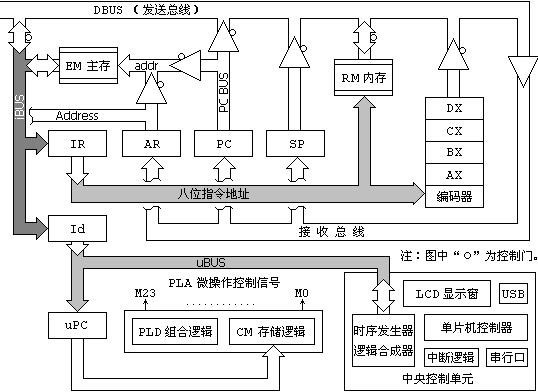
\includegraphics[width=0.9\linewidth]{1.jpg}
  \caption{数据通路}
  \label{fig:1}
\end{figure}

\subsection{指令寄存器 IR}

IR 框由 2 片 74LS574 锁存器构成 16 位指令寄存器,主要用于存放指令的操作码与操作数,它的输入端经指令总线(IBUS)分别与主存和数据总线构成取数通路。其锁存输出端编码产生通用寄存器地址,并指定由 IR15~IR8 提供内存地址。

\subsection{指令寄存器 ID}

ID 框由指令编译电路(CPLD)构成 11 位微地址寄存器,主要用于存放指令排序器所定义的指令起始微地址(亦可称为指令的微程序入口地址)。ID 的输入端经指令总线(IBUS)分别与主存和数据总线构成取数通路。其三态输出端经微总线(BUS)单向流入微程序计数器的输入端口,在时序电路的控制下形成与当前指令相对应的微程序入口地址。

由指令排序格式可知,本装置微控制器在“取指”时按“字节”排序,指令系统微程序入口地址的寻范围为 600~7FFh,最多可支撑 256 条指令的微运行,其容纳率达通用计算机控制器的设计水准。控制器支持指令的变长编码,在模型机的设计与实现中,可根据指令的容纳率动态编制与确定机器指令中操作码的长度(简称指令段)。指令段通常存放在机器指令起始字节的高端。在取指时用“与逻辑”保留指令段屏敝地址段,例如设计一个八条以下的指令系统模型机,它的指令段长度为三位,存放在机器指令起始字节的“D7~D5”位置,可产生 7C0h、780h、740h、700h、6C0h、680h、640h、600h 共八个微程序入口地址,分别对应机器指令的 E0h、C0h、B0h、80h、60h、40h、20h、00h。


这里仅阐述了指令系统起始微入口的形成途径与排序格式,它的执行涉及微控制器原理,我们按排在微控制器实验中进行。



\section{实验步骤}

\begin{itemize}
  \item 调整 pc
  \item 实现 $IO \rightarrow BUS$
  \item $BUS \rightarrow IR$
  \item 显示下址
\end{itemize}

\section{调试过程、结果与分析}

input输入数据到指令寄存器

\begin{figure}[h]
  \centering
  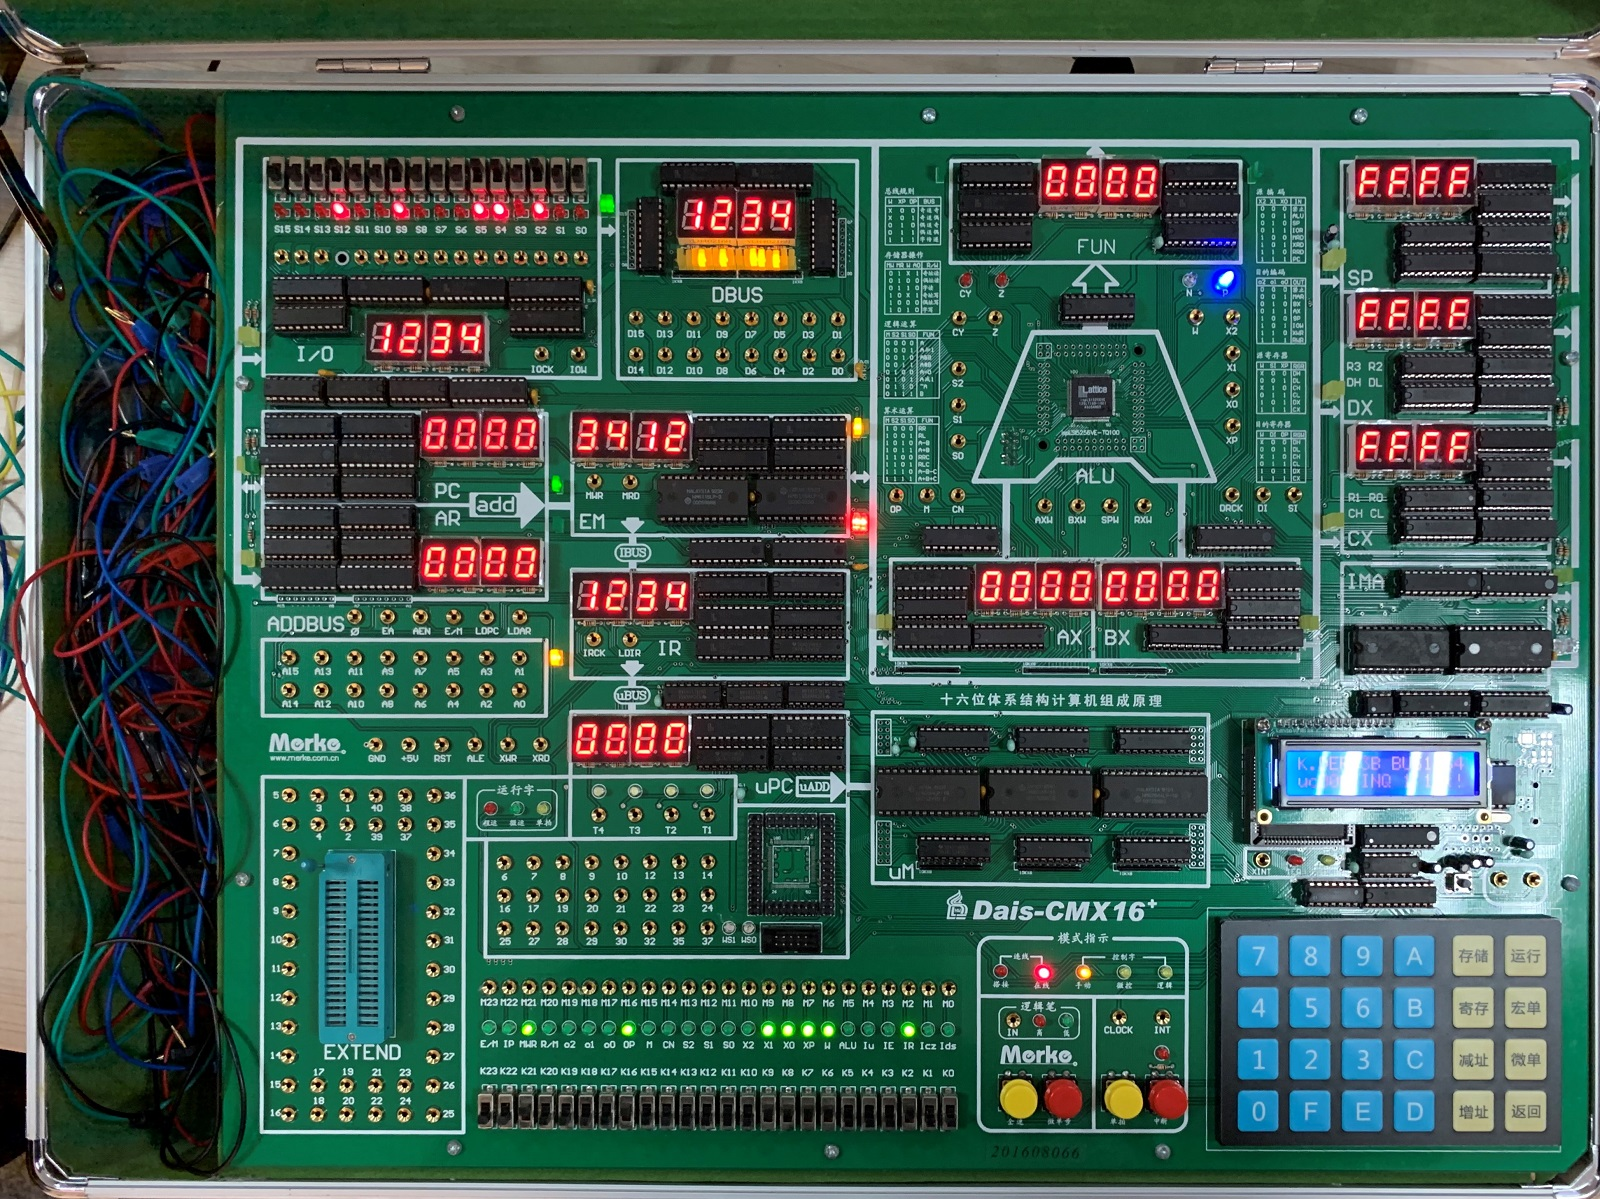
\includegraphics[width=0.9\linewidth]{2.jpg}
  \caption{输入到指令寄存器}
  \label{fig:2}
\end{figure}

更换in值并将第一个存入的数输入到IR(MWR=0,K2=1)s

\begin{figure}[h]
  \centering
  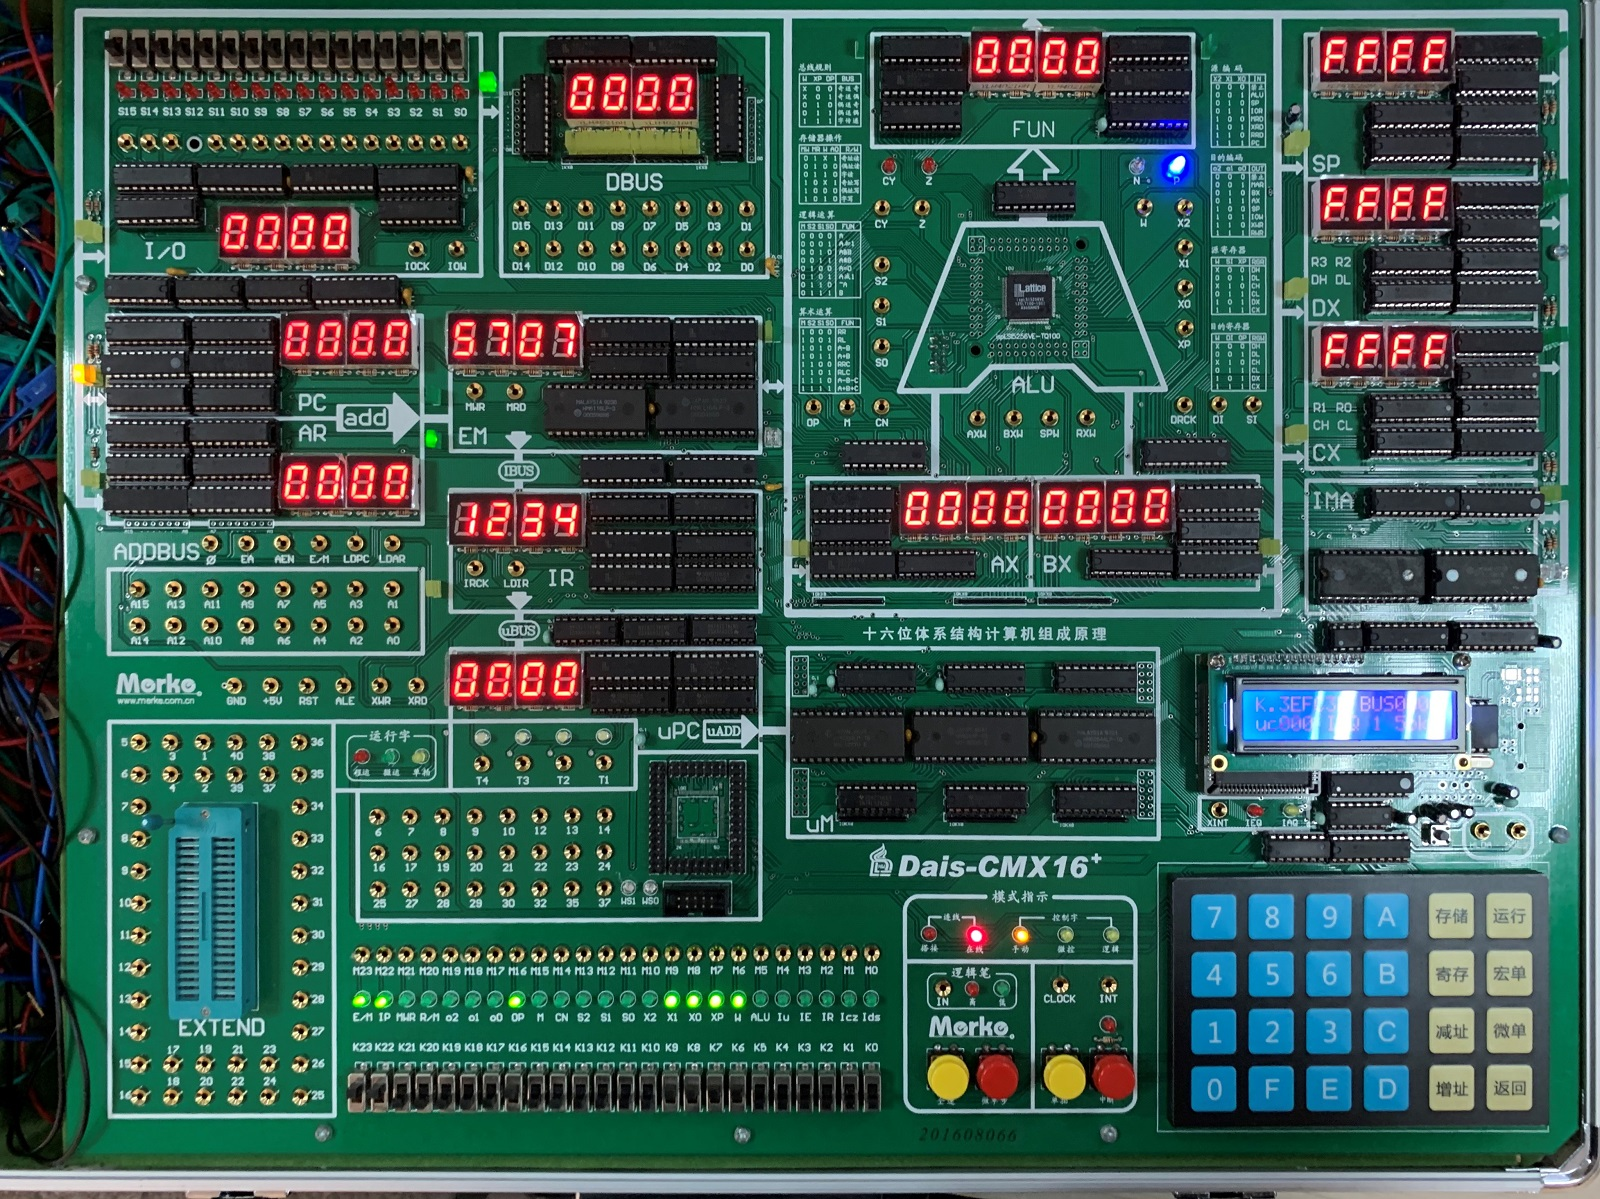
\includegraphics[width=0.9\linewidth]{3.jpg}
  \caption{输入到IR}
  \label{fig:3}
\end{figure}

\begin{figure}[h]
  \centering
  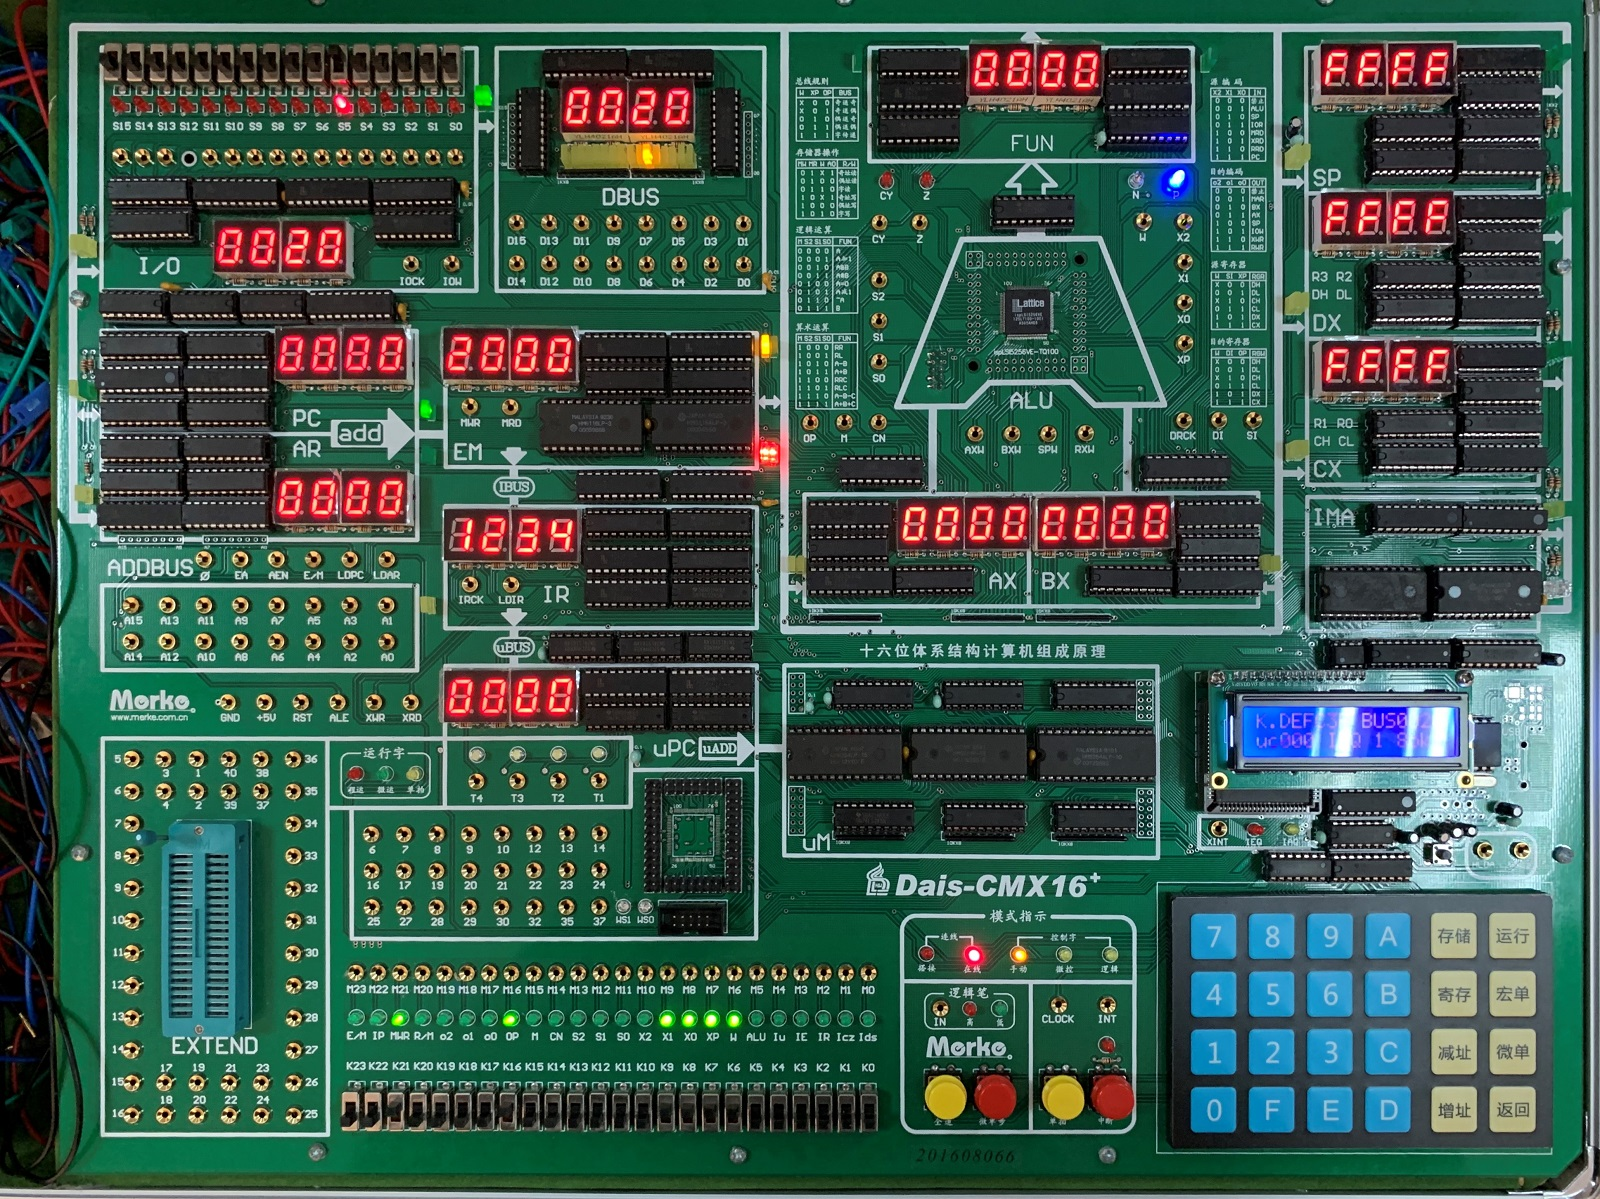
\includegraphics[width=0.9\linewidth]{4.jpg}
  \caption{输入到IR 2}
  \label{fig:4}
\end{figure}

\begin{figure}[h]
  \centering
  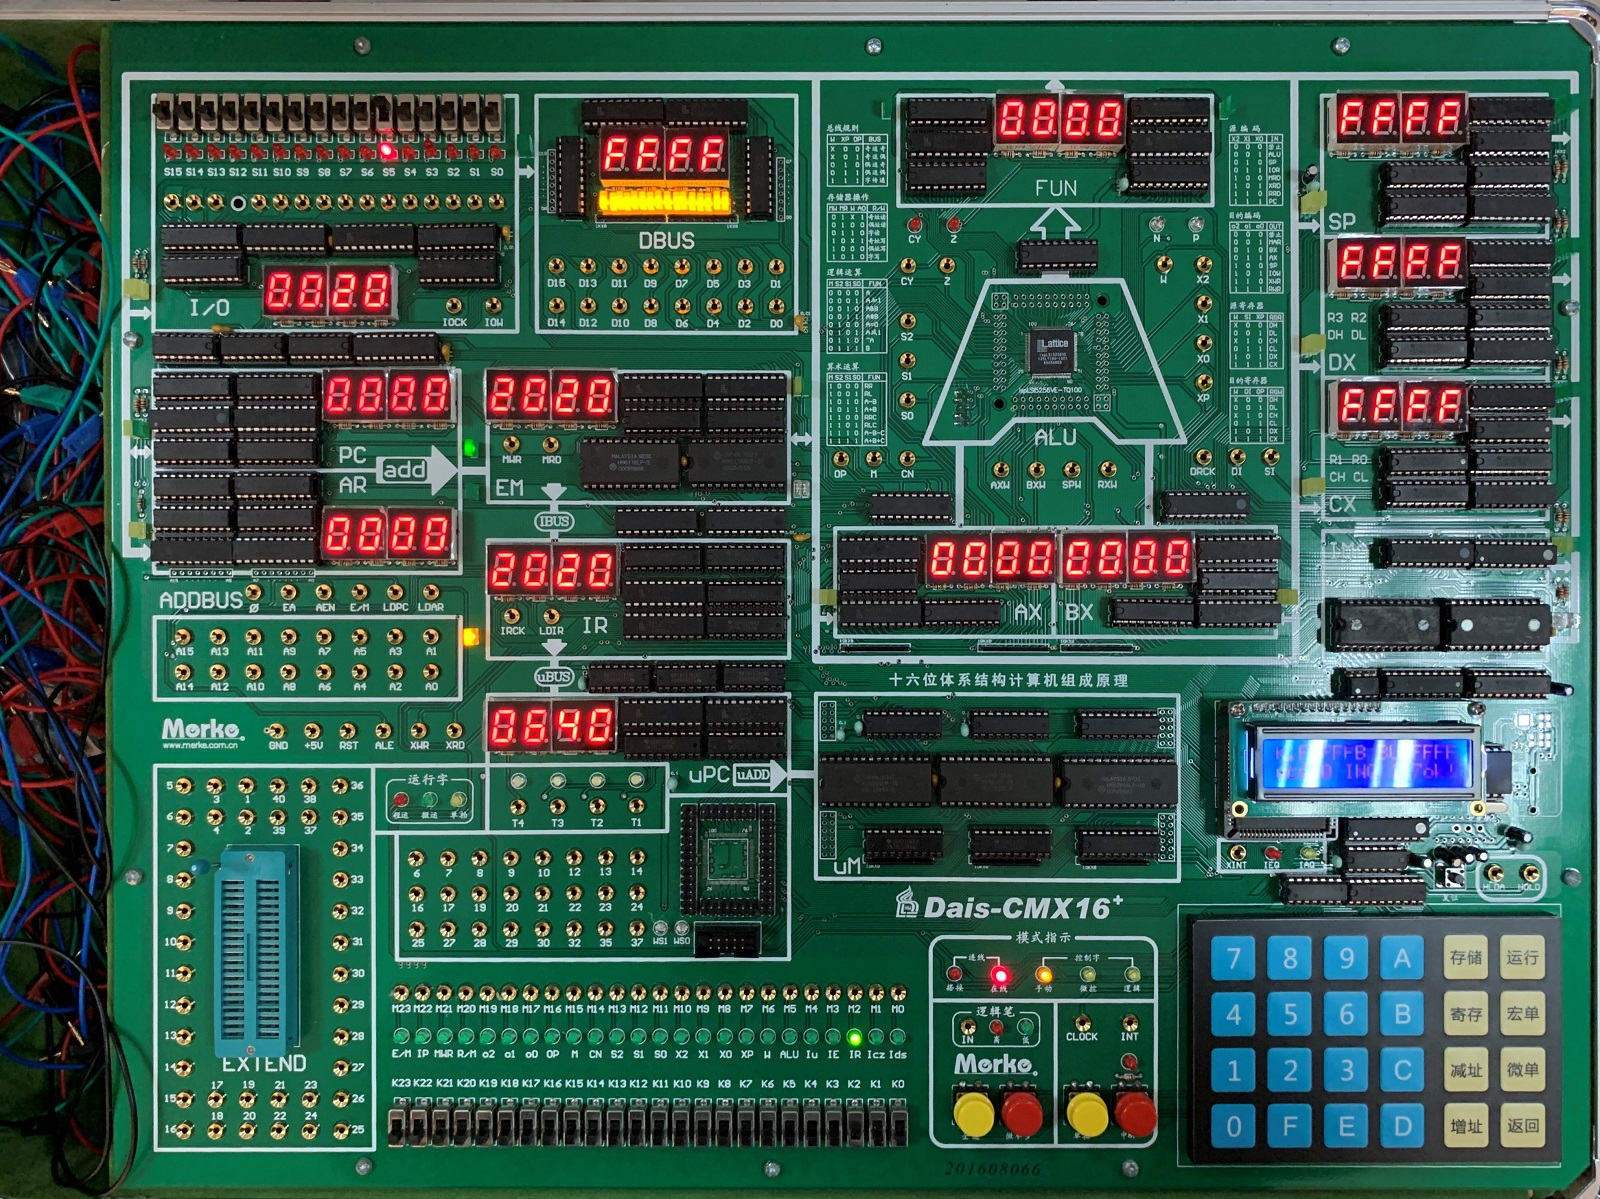
\includegraphics[width=0.9\linewidth]{5.jpg}
  \caption{输入到IR 3}
  \label{fig:5}
\end{figure}


\section{总结}

本次实验使用在线模式,有了极大的便利。实验过程中须注意要及时调整MWR和K2的值,
下表为部分下址:

\begin{tabular}{|c|c|c|}
  \hline 
  IR & 下址 \\ \hline
  0020 & 0640 \\ \hline
  0001 & 0602 \\ \hline
  0002 & 0604 \\ \hline
  0040 & 0680 \\ \hline
  
\end{tabular}

\section{附件}

\end{document}
